\documentclass[a4paper,fleqn]{cas-dc}
\usepackage[numbers,sort&compress]{natbib}
\usepackage{amsmath,amssymb,booktabs,microtype}
\usepackage{graphicx,xr,xurl}
\hypersetup{pdfauthor={Meshaal Mouawad},pdfsubject={Half-moon classification and representation loss},pdfcreator={LaTeX3; cas-dc.cls; hyperref.sty}}
\externaldocument{Supplement_labels}
\graphicspath{{../Figures/}}
\newcommand{\R}{\mathbb R}
% Use the publisher's nologo title option to keep the submission source flat.
\ExplSyntaxOn
\keys_set:nn { stm / mktitle } { nologo = true }
\ExplSyntaxOff
% V12 reader-first revision. V11 experimental and mathematical records are preserved.
\newcommand{\HalfMoonIntroduction}{%
\section{Introduction}\label{sec:introduction}
Direction normalization is useful when orientation matters more than magnitude: it suppresses variation in distance from a reference origin. That same operation can destroy class information when distance matters. The half-moon task makes the conflict concrete. Its two classes occupy thick semicircular bands---an upper half-ring and a translated lower half-ring---whose positions determine whether they are disjoint or overlap (Fig.~\ref{fig:geometry}). We establish that direction alone loses class information at every origin for specified arrangements and that one near/far radius bit restores the decisions in a disjoint case.

At vertical displacement $h=0.5$, take the midpoint origin $c=(0.5,0.25)$. The class-0 point $x_0=(1,0.25)$ and class-1 point $x_1=(2,0.25)$ both lie inside their respective half-rings. Each lies directly to the right of $c$, so their normalized directions coincide at $(1,0)$ despite opposite labels. Their distances from $c$ are $0.5$ and $1.5$; a near/far threshold of $0.8$ distinguishes them. This constructed example explains one lost decision, not a positive population error. The proof below establishes conflicting decisions on a set of directions with positive measure, and does so for every origin.

We quantify the loss with \emph{Bayes risk}: the lowest possible misclassification probability when the class distributions are known and the classifier makes the best decision permitted by its input. Comparing this ideal error for raw coordinates with that for directions isolates information removed by preprocessing. The difference is distinct from the extra error of a trained network using finite data and an imperfectly learned decision rule. It also defines a harder question than whether a few chosen origins give poor accuracy: can \emph{any} origin, including one arbitrarily far away, remove the representation-induced error?

Spatial-sign preprocessing and geometric classifiers already use normalized directions \citep{Serneels2006,Graf2003}. Decision-sufficiency theory establishes when a transformation retains optimal class decisions \citep{Silva2012,Silva2024,Gyorfi2023}, while recent \emph{Pattern Recognition Letters} studies connect classification performance to feature geometry and normalization \citep{Poblete2026,Ahmadian2025}. The unresolved geometric question for the present populations is whether these decisions can be preserved by moving a shared origin, and what restricted radial information would recover them when they cannot.

We answer it by deriving the probability of opposing decisions merged along each ray, proving a uniform distant-origin limit to orthogonal-projection risk, and constructing explicit positive lower bounds over the whole plane. A common-threshold radius bit then selects between two angular decisions and exactly recovers the labels in one disjoint half-moon configuration; the admissible threshold interval also determines its radius-error tolerance. Controlled neural experiments test how close learned decisions come to the corresponding population risks, using 500 candidate fits and 250 selected evaluations across the main and repair studies.
}

\newcommand{\HalfMoonBackground}{%
\section{Background and related work}\label{sec:background}
\paragraph{Representations and achievable classification error.}
A preprocessing map determines what information a classifier can use. The spatial-sign map of an observation $x$ about a shared origin $c$ is $T_c(x)=(x-c)/\|x-c\|$ for $x\ne c$: it reports a unit direction and ignores the radius $\rho=\|x-c\|$ \citep{Serneels2006}. Direction and radius together recover the original point by $x=c+\rho T_c(x)$. Retaining both therefore supplies a full-information control. A Bayes classifier selects the most probable label given the supplied input. Its Bayes risk is the residual probability of error even under that optimal rule. A larger Bayes risk after normalization means that the representation itself prevents some correct decisions; a neural model cannot recover them by more training.

\paragraph{What earlier geometric and normalization studies establish.}
Spatial-sign preprocessing and normalized-feature classification establish ways to compare directions \citep{Serneels2006,Graf2003}. In \emph{Pattern Recognition Letters}, Poblete et al.~\citep{Poblete2026} compare classifier rules on fixed learned features across eight datasets: rankings vary with geometry, while the predicted directional association of radial compatibility is unsupported. Their evidence concerns choosing a rule for an existing representation. Ahmadian and Lindsten~\citep{Ahmadian2025} evaluate activity novelty detection with radial kernels, normalization and quantization; their ablations report different performance for normalized and unnormalized variants. These observations motivate a sharper question: before fitting any classifier, can a change of normalization origin prevent the loss of optimal class decisions?

\paragraph{Decision preservation and radial information.}
Silva and Narayanan~\citep{Silva2012} analyze representation quality through Bayes and learned error; later decision-sufficiency results distinguish preserving a label distribution from preserving the decision that minimizes a given loss \citep{Silva2024,Gyorfi2023,Silva2025}. Dubois et al.~\citep{Dubois2021} identify unit direction as an invariant of positive scaling. The key condition is intuitive: points collapsed to the same direction must require the same optimal decision for direction alone to be sufficient. Our half-moons supply a continuous geometry in which that condition can fail and in which the normalization origin itself varies.

A representation can instead preserve only the extra information needed for the decision. Bayes-aware quantization and learned cut points investigate compressed decision inputs \citep{OehlerGray1995,Senozan2024}. Our repair asks a precise question: can \emph{one shared near/far radius threshold}, combined with the retained direction, preserve decisions across both continuous class regions? The threshold then acts as a minimal decision cue rather than a measurement that reconstructs the full observation.

\paragraph{Why all origins require a separate analysis.}
Projection methods study the error incurred by a selected lower-dimensional view \citep{Hamsici2007,Hamsici2008,Oh2025}. From a very distant origin, rays crossing a bounded population become nearly parallel, and normalized direction approaches an orthogonal projection in its decision-making effect \citep{Orponen2019}. Thus proving positive loss for each finite origin alone does not settle whether the infimum over \emph{all} origins is positive. Finite planar separability geometry provides another ingredient: connected regions whose convex hulls intrude into each other cannot always be isolated into different directional sectors \citep{Hurtado2001}. We combine these geometric observations with population risk to establish both finite-origin loss and its strictly positive global floor, then ask how a restricted radius code changes that conclusion.
}

\newcommand{\HalfMoonDiscussion}{%
\section{Discussion}\label{sec:discussion}
The experiments distinguish error already present in the original coordinates, additional error forced by direction-only preprocessing, and excess error from fitting a network. In the disjoint midpoint condition, the small learned excess over the Bayes floor (Table~\ref{tab:neural-main}) shows that most direction-only errors arise from the input representation. In the overlapping condition, raw-coordinate ambiguity already exists and normalization adds further loss. Accuracy comparisons alone would not reveal these two mechanisms.

Poblete et al.~\citep{Poblete2026} show that classifier rankings depend on the geometry of fixed learned features; our all-origin criterion instead determines when \emph{no} classifier can recover decisions removed by direction normalization. Ahmadian and Lindsten~\citep{Ahmadian2025} document normalization-sensitive novelty-detection performance; our Bayes-risk analysis isolates representation loss before learning. Relative to decision-preservation theory \citep{Silva2012,Silva2024,Gyorfi2023}, the ray-cancellation identity and distant-origin limit give a geometric test for a whole family of normalization maps, including origins receding to infinity.

The one-bit result specifies the information needed to repair the disjoint midpoint geometry. Radius alone has $50\%$ Bayes error under the equal-prior reflected sampling laws, yet its near/far bit selects between two angular separators when combined with direction. The certified threshold interval applies to the explicit decoder; the independent neural evaluation shows how closely a trained model uses that representation, without equating its few residual errors with the decoder's exact guarantee. The resulting evaluation sequence is to identify the retained class information, calculate its optimal risk, and then assess learning error relative to that risk.
}

\begin{document}
\let\WriteBookmarks\relax
\renewcommand{\printorcid}{}
\shorttitle{Global loss bounds and one-bit recovery}
\shortauthors{M. Mouawad}
\title[mode=title]{Global loss bounds and one-bit recovery for direction-normalized half-moons}
\author[1]{Meshaal Mouawad}
\cormark[1]
\ead{mm4922@msstate.edu}
\affiliation[1]{organization={Department of Electrical and Computer Engineering, Mississippi State University},addressline={216 Simrall Hall, 406 Hardy Road},city={Mississippi State},state={MS},postcode={39762},country={USA}}
\cortext[1]{Corresponding author.}
\begin{abstract}
Normalizing a point to unit direction from a chosen origin discards its distance, which may carry information needed to classify it. We study the resulting loss in two crescent-shaped half-moon populations and ask whether moving the origin can preserve the missing decisions. We compare Bayes risks, the minimum attainable classification errors from raw coordinates and from direction alone. For absolutely continuous binary populations in dimension at least two, directional risk at distant origins converges uniformly to orthogonal-projection risk. Geometric criteria and computable lower certificates then establish positive classification loss for every origin in specified disjoint and overlapping half-moon configurations. In one disjoint configuration, adding a near/far radius bit to direction restores every class decision; an exact threshold interval determines the sharp tolerance to bounded radius-measurement error. Controlled neural studies comprise 500 candidate fits and 250 selected evaluations. In the independent repair experiment, direction-only networks made 54,362 errors in 500,000 observations ($10.8724\%$), whereas networks with the extra bit made three ($0.0006\%$). These results distinguish preprocessing-induced error from learned error and establish a minimal radial repair for the constructed geometry.
\end{abstract}
\begin{keywords}
Direction normalization \sep Bayes risk \sep Half-moon classification \sep Spatial sign \sep Radial quantization \sep Neural networks
\end{keywords}
\maketitle
% Keep short multi-line mathematical definitions on a single page.
\interdisplaylinepenalty=10000
\hypersetup{pdfauthor={Meshaal Mouawad},pdfsubject={Half-moon classification and representation loss},pdfcreator={LaTeX3; cas-dc.cls; hyperref.sty}}
\HalfMoonIntroduction
\begin{figure*}[t]
\centering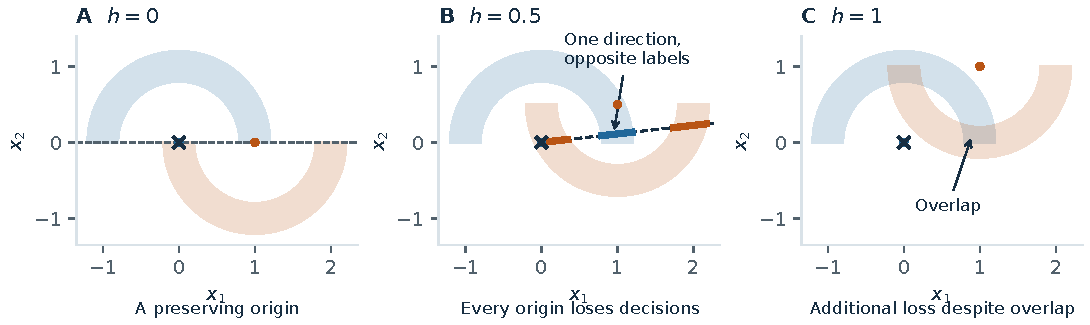
\includegraphics[width=\textwidth]{Fig1_Geometry.pdf}
\caption{Half-moon geometry and the effect of radial removal. Blue and orange indicate the two class supports; crosses mark the illustrated origin. The vertical displacement between class centers is $h$. (A) At $h=0$, the vertical direction preserves the label (the neural negative control uses $h=-0.25$). (B) At $h=0.5$, one illustrated ray crosses both labels; the theorem establishes positive loss for every origin. Colored ray segments are exact support intersections. (C) At $h=1$, the original classes overlap, and normalization adds further ambiguity. The diagrams explain the mechanism; population risks are computed separately.}\label{fig:geometry}
\end{figure*}
\HalfMoonBackground
% Main-text fragment; supplementary proofs are in supplement_theory.tex.
% Requires amsmath, amssymb, booktabs and natbib.
\section{Half-moon geometry and the minimum error after normalization}
\label{sec:origin-theory}

To determine what is lost by retaining direction alone, we first describe the class regions and the best possible decision before and after normalization. Each half-moon is a thick semicircular ring, bounded by an inner and an outer radius. Class 0 occupies an upper half-ring centered at the origin; class 1 occupies a lower half-ring whose center is shifted one unit to the right and $h$ units upward. The displacement $h$ controls the separation or overlap of the two bands (Fig.~\ref{fig:geometry}). An origin $c$ determines the rays along which distinct points are merged when their distance is discarded. We calculate the class probability merged on each ray and then ask whether any choice of $c$ can avoid the resulting minimum classification error.

\begin{samepage}
Let $a=0.8$, $b=1.2$, $m_0=(0,0)$ and $m_1=(1,h)$, where $h$ is the upward center displacement. The open class supports are
\begin{align}
 S_0&=\{x:a<\|x\|<b,\ x_2>0\},\nonumber\\
 S_1&=\{x:a<\|x-m_1\|<b,\ x_2<h\}.
 \label{eq:halfmoon-supports}
\end{align}
\end{samepage}
Each support has area $H=\pi(b^2-a^2)/2=2\pi/5$. The primary generator draws points uniformly over the area of each band, so its density is $f_i^A=\mathbf1_{S_i}/H$. A second sampling law draws radius and angle uniformly instead, giving $f_i^R(x)=\mathbf1_{S_i}(x)/[\pi(b-a)\|x-m_i\|]$; these laws allocate different probability mass within the same geometry. Experiments use equal class priors. The geometric positivity results apply to any positive priors $\pi_i$ and densities positive almost everywhere on the respective supports.

\paragraph{Why one ray can force classification error.}
A classifier that sees the original coordinates may give different labels to points at different distances along the same ray. After normalization it sees only the angle and must make one decision for all of them. To count the probability of the conflicting decisions, define the signed density $d=\pi_0f_0-\pi_1f_1$: its positive and negative regions favor classes 0 and 1, respectively. Let $u_\theta=(\cos\theta,\sin\theta)$ and $[z]_+=\max(z,0)$. Integration along the ray from $c$ uses the polar area factor $r$, because an angular slice contains more area at a larger radius. The opposing class-preference masses on that ray are
\begin{equation}
\begin{aligned}
 A_c(\theta)&=\int_0^\infty[d(c+ru_\theta)]_+r\,dr,\\
 B_c(\theta)&=\int_0^\infty[-d(c+ru_\theta)]_+r\,dr.
\end{aligned}
\label{eq:ray-masses-main}
\end{equation}
Let $R_X^*$ and $R^*_{T_c}$ denote the minimum classification risks from raw coordinates and directions, respectively. Using the masses in~\eqref{eq:ray-masses-main}, the binary Bayes-risk identity yields
\begin{equation}
 \Delta(c):=R^*_{T_c}-R_X^*
 =\int_0^{2\pi}\min\{A_c(\theta),B_c(\theta)\}\,d\theta.
 \label{eq:ray-loss-main}
\end{equation}
The smaller mass on each ray is the probability that even the best direction-only decision cannot retain from the raw-coordinate Bayes rule. Integrating it over angles gives the additional Bayes risk $\Delta(c)$. Thus loss occurs when a nonzero set of directions merges regions preferring opposite labels. This specializes decision-preservation theory \citep{Silva2012,Silva2024} to a moving normalization origin; Supplementary Section~\ref{supp:bayes} derives the identity.

\paragraph{Theorem 1: loss at every finite origin.}
A collision seen from one origin might disappear when the origin moves. The stronger question is whether some viewpoint separates the two half-rings into different sets of directions. Their geometry answers that question for the positive displacements below: despite disjoint original class regions, every finite viewpoint merges conflicting decisions. For $0<h\leq\sqrt{3/5}$, the supports have disjoint interiors and
\begin{equation}
 R_X^*=0,\qquad \Delta(c)>0
 \quad\text{for every }c\in\mathbb R^2.
 \label{eq:all-origin-disjoint}
\end{equation}
At $h=0$, every origin with $c_2=0$ preserves zero risk. More generally, for $h<0$, origins in the separating strip $h\leq c_2\leq0$ preserve zero risk. At $h=1$, the supports overlap and
\begin{equation}
 R_X^*>0,\qquad \Delta(c)>0
 \quad\text{for every }c\in\mathbb R^2.
 \label{eq:all-origin-overlap}
\end{equation}

\emph{Proof idea.}
Horizontal slicing shows that the disjoint supports satisfy $\sqrt{a^2-h^2}\geq1/5$ in the stated range. Yet each connected half-ring intrudes into the other one's convex hull. Were their directional images disjoint from some origin, a separating angular cone would contain one region's convex hull while excluding the other, contradicting this intrusion. This adapts the geometry of Hurtado et al.~\citep{Hurtado2001}; positive class densities convert the forced angular overlap into positive risk in~\eqref{eq:ray-loss-main}. At $h=1$, the same argument uses connected class-exclusive regions to establish additional loss despite the overlap already present in raw coordinates. Supplementary Sections~\ref{supp:geometry}--\ref{supp:overlap} provide the explicit geometric witnesses, inequalities and complete proofs.

% Suggested main-text replacement/extension for the old positive-infimum theorem.
% The supplement fragment defines supp:projection-boundary.
\paragraph{Theorem 2: the decision problem at distant origins.}
An origin can move without bound, so positive error at each fixed viewpoint does not automatically imply a positive worst-case floor over all possible origins. Seen from far away, the rays through a bounded class population become nearly parallel: their direction-based decisions approach those allowed by projecting the population onto a line perpendicular to the viewing direction (or onto a perpendicular hyperplane in higher dimensions). This is the relevant boundary case of radial projection \citep{Orponen2019}. We therefore compare the optimal classification risks, not merely the geometric images. For binary populations with densities in dimension $n\geq2$, fix a reference point $p$, let $e$ be a unit viewing direction, and let $P_e$ denote orthogonal projection onto the hyperplane perpendicular to $e$. Then
\begin{equation}
 \lim_{R\to\infty}\sup_e
 \left|R^*_{T_{p+Re}}-R^*_{P_e}\right|=0.
 \label{eq:projection-limit-main}
\end{equation}
Write $\Delta_\infty(e)=R^*_{P_e}-R_X^*$. The loss surface, completed by these projection limits, is continuous on a compact domain. Consequently,
\begin{equation}
 \inf_c\Delta(c)>0
 \quad\Longleftrightarrow\quad
 \begin{cases}
 \Delta(c)>0&\text{all finite }c,\\
 \Delta_\infty(e)>0&\text{all directions }e.
 \end{cases}
 \label{eq:global-criterion-main}
\end{equation}
Thus optimizing the origin cannot make loss vanish when both finite radial views and all limiting linear projections lose decisions.

\emph{Half-moon consequence.}
The connected winner regions in Theorem~1 have overlapping projection intervals in every direction. Equations~\eqref{eq:projection-limit-main}--\eqref{eq:global-criterion-main} therefore strengthen its conclusion to
\begin{equation}
 \inf_{c\in\mathbb R^2}\Delta(c)>0
 \quad\text{for }0<h\leq\sqrt{3/5}\text{ and for }h=1.
 \label{eq:global-positive}
\end{equation}
This holds for every fixed pair of positive priors and densities positive almost everywhere on their respective supports. The proof controls signed probability mass in total variation, so it establishes convergence of the optimal decision risk. Supplementary Section~\ref{supp:projection-boundary} proves the general result and gives an explicit convergence bound for bounded-support densities of bounded variation.

% Standalone main-text replacement paragraph. Definitions of d and Delta precede it.
\paragraph{A numerical lower certificate for the whole plane.}
The preceding result establishes a strictly positive loss floor, but a numerical certificate must still say how large a loss is guaranteed regardless of origin. Such a bound can be constructed from two interior regions where one class is favored by a fixed probability margin. Their relative positions make conflicting rays unavoidable, while their sizes bound the amount of probability merged on those rays. In the plane, let $K_+,K_-$ be compact connected cores whose radius-$\rho$ neighborhoods satisfy $d\geq\kappa_+>0$ and $d\leq-\kappa_-<0$, respectively. Suppose each core meets the other's convex hull, their convex hulls contain a common disk $B(p,\delta)$, and both cores lie within distance $M$ of $p$. Writing $\kappa=\min(\kappa_+,\kappa_-)$ gives
\begin{equation}
 \inf_c\Delta(c)\geq\kappa\min\left\{
 \frac{\sqrt3\rho^3}{6M},\;2\rho\delta\right\}>0.
 \label{eq:constructive-global}
\end{equation}
For bounded origins, mutual convex-hull intrusion forces rays through both cores; their neighborhoods provide an angular interval with conflicting class mass. For distant origins, the shared convex-hull disk supplies the bound. Thus the certificate does not rest on a finite search grid. Supplementary Section~\ref{supp:constructive-global} proves the result and optimizes the split between these regions. For equal-prior area sampling, optimized whole-plane lower certificates exceed $0.0205$ percentage points (pp) at $h=0.5$ and $0.00119$~pp at $h=1$. Eroded half-annuli provide such cores throughout the disjoint regime of Theorem~1 under both sampling laws and any fixed positive priors.

\paragraph{Computing the best possible error at a chosen origin.}
An ideal directional classifier needs no neural training: for each viewing angle, one can integrate the class probabilities carried by that direction and choose the more probable label. For the half-annuli, circle tangencies and boundary intersections partition directions into finitely many cells. Radial support order is fixed inside a cell, so one representative ray determines whether opposite preferences coexist. Exact radial primitives then reduce Bayes risk to one angular integral. Ball arithmetic and a bounded-variation truncation bound certify its value. Supplementary Sections~\ref{supp:finite}--\ref{supp:bv} give the finite preservation test, integration formulas and error bounds. At equal priors, the density ratio $f_i^R/f_i^A\in[5/6,5/4]$ also gives $\Delta_R(c)\geq(5/6)\Delta_A(c)$.

\paragraph{Recovering the decision with one radius bit.}
The all-origin loss result rules out fixing the midpoint case by moving the origin, but it leaves open whether a small amount of distance information can repair the representation. The proposed bit answers only whether an observation is near or far from the fixed midpoint; it does not report the full distance. At $h=0.5$, direction alone has positive loss at every origin. At $c=(1/2,1/4)$, append $q=\mathbf1\{\|x-c\|>4/5\}$. For $q=0$, the sign of $9u_1+10u_2$ determines the class; for $q=1$, the sign of $u_2-u_1$ determines it. Positive signs identify class~0. Figure~\ref{fig:bit-repair} shows how the radial bit assigns observations to the two angular rules. Together, the two rules correctly label the complete class supports under their respective bit conditions, giving zero Bayes risk under either sampling law and any positive priors. Supplementary Section~\ref{supp:one-bit} proves the separating inequalities. Since zero additional radial bits leave the positive direction-only floor, one bit is the minimal radial addition at this geometry.

\paragraph{How accurately must radius be measured?}
The threshold is not an arbitrary tuned parameter: the geometry permits a complete interval of shared near/far cutoffs that retain every decision. With the same angular rules, recovery is exact precisely for $\alpha\leq t\leq\beta$, where $\alpha\approx0.7433034374$ and $\beta\approx0.8120914734$ (Threshold Addendum, Proposition~1). If the measured radius is $\widehat r=r+e$, $|e|\leq\varepsilon$, every support label is preserved for every admissible error function exactly when
\begin{equation}
\alpha+\varepsilon\leq t\leq\beta-\varepsilon.
\label{eq:radius-error}
\end{equation}
The midpoint threshold $t_\star=(\alpha+\beta)/2\approx0.7776974554$ maximizes the guaranteed tolerance at $(\beta-\alpha)/2\approx0.0343940180$ (Addendum, Corollary~1). The neural experiments retain $t=0.8$.

\begin{figure*}[t]
\centering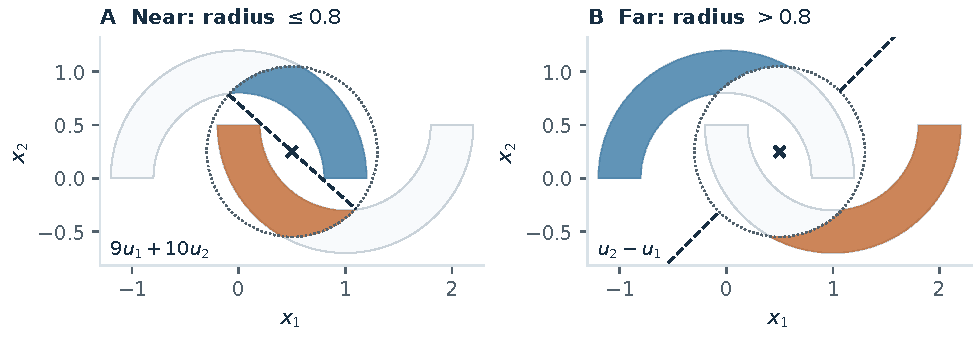
\includegraphics[width=.84\textwidth]{Fig2_One_Bit_Recovery.pdf}
\caption{Exact one-bit recovery at $h=0.5$. The same radius threshold, $0.8$ about $c=(0.5,0.25)$, applies to every direction. (A) Inside the threshold, $9u_1+10u_2$ separates the two classes. (B) Outside it, $u_2-u_1$ separates them. Blue denotes class 0 and orange class 1. Each panel shows the portion of the original supports assigned to that radial code; the dashed line is its angular decision boundary. Direction together with the bit determines the class.}\label{fig:bit-repair}
\end{figure*}
% Experimental sections drawn only from the frozen and audited neural study.
% Requires booktabs and natbib. Add experimental_references.bib to the bibliography.
% Invoke \HalfMoonExperiments in the main text; place
% \HalfMoonExperimentalLimitations inside the consolidated limitations section.

\newcommand{\HalfMoonExperiments}{%
\section{Controlled neural experiments}
\label{sec:experiments}

\subsection{Design and evaluation}
Bayes risk describes the error permitted by an input representation even for an ideal classifier. Our neural experiment asks how closely a trained network approaches that floor and whether changing the normalization origin changes its actual errors. We therefore hold the learner and data-generation conditions fixed while varying what information it receives. Equal-prior observations were sampled uniformly in area from half-annuli with radii $0.8$ and $1.2$, centered at $(0,0)$ and $(1,h)$, for $h\in\{-0.25,0.5,1\}$. Each of ten independent dataset/initialization seeds, numbered 1001--1010, supplied balanced training, validation and test sets of 2,000, 2,000 and 50,000 observations. Within each geometry/seed, conditions shared observations; initializations were paired across conditions and geometries. Data-generation phases, geometries and splits used distinct streams.

The five inputs isolate what the classifier receives. Raw coordinates $R$ preserve the original position. Direction-only inputs $D_0$, $D_M$ and $D_A$ discard radius about three origins: $(0,0)$, the midpoint $(0.5,h/2)$ and the upper origin $(0,3)$. The control $P_A$ retains both direction and radius about $(0,3)$, which together reconstruct the original coordinates. Directions use exact division by the nonzero norm, with zero residual mapped to zero. All inputs are then standardized from training-set means and population standard deviations; constant features use scale one. This positive affine transformation retains the information in each representation.

The same network architecture was used to separate input-information effects from changes in model capacity: 64 tanh hidden units and a linear output. We fitted class labels $-1/+1$ using mean squared error (MSE), assigning positive outputs to the second class. Full-batch Adam~\citep{Kingma2015} used $(\beta_1,\beta_2)=(0.9,0.999)$, optimizer $\epsilon=10^{-8}$, and learning rates $0.001$ and $0.01$. Every candidate executed 4,000 updates.\footnote{The stopping criterion was completion of the fixed update budget, including candidates whose selected checkpoint occurred earlier.} Validation was evaluated at initialization and every 50 updates. Selection minimized validation error, followed by validation MSE, earlier update and lower learning rate.

The main design required 300 candidate fits. At $h=1$, width-15 and unconditioned width-64 diagnostics each added 60 fits for $R,D_A,P_A$. These 420 final candidate fits were separate from a 48-fit development stage using seeds 101 and 103. Training and analysis protocols were frozen before final test generation; the 210 selected models were then evaluated once. 

Misclassification error was the primary outcome; accuracy, MSE and the gap between learned error and the representation's Bayes floor were secondary. Six planned paired contrasts compared the midpoint and upper-origin direction errors with zero-origin direction error at each displacement ($D_M-D_0$ and $D_A-D_0$). The inference unit was the independently repeated dataset/initialization seed, not the individual test observation. We summarized paired seed differences using their mean, sample standard deviation and Student-$t$ intervals with nine degrees of freedom. Simultaneous 95\% intervals used $t_9(1-0.05/12)$ for the six-contrast family. Supplementary results retain whole-seed bootstrap sensitivity analyses and pointwise diagnostic intervals.

The analytical Bayes rule was evaluated on the identical test observations. Class-specific errors and class-stratified Monte Carlo standard errors separated test sampling from numerical integration bounds and between-seed variation. Across the 15 main conditions, mean empirical Bayes-rule error differed from integrated risk by at most $0.061$ percentage points (pp).

\subsection{Results}
The key comparison is between the attainable error in each input representation and the corresponding fitted-network error (Table~\ref{tab:neural-main}). Learned errors were close to their representation-specific floors: the largest mean excess among 15 principal conditions was $0.471$ percentage points (pp). At $h=0.5$, raw and direction-plus-radius inputs produced zero observed test errors, whereas direction-only inputs incurred errors consistent with their positive population floors. At $h=1$, $R$ and $P_A$ achieved $6.790\%$ and $6.833\%$ error against their common $6.716\%$ floor.

All five nonzero primary origin contrasts had simultaneous intervals excluding zero (Supplementary Table~\ref{tab:neural-contrasts}). The midpoint reduced error relative to the zero origin in both nonlinear configurations. The upper origin increased error by $9.379$~pp at $h=0.5$ and decreased it by $1.445$~pp at $h=1$. For $h=-0.25$, $D_M-D_0$ was zero for every seed. Thus the effect of changing origin followed the class arrangement.

The paired $P_A-R$ difference at $h=1$ was $0.044$~pp, with a pointwise 95\% interval $[-0.043,0.130]$. All three width-15 versus width-64 diagnostic intervals included zero. Removing affine conditioning increased $D_A$ error by $0.179$~pp, $[0.053,0.305]$; the corresponding $R$ and $P_A$ intervals included zero. Complete seed outcomes, signed excess estimates, prediction arrays and learning histories accompany the experiment.

\HalfMoonMainRiskTable

}

\newcommand{\HalfMoonMainRiskTable}{%
\begin{table}[t]
\centering\small
\setlength{\tabcolsep}{3pt}
\caption{Population Bayes risk and neural test error. Errors are mean $\pm$ sample SD over ten seeds; excess is mean error minus Bayes risk. Risk and error are percentages; excess is in percentage points. $R$ denotes raw coordinates, $D$ direction, and $P$ direction plus radius; subscripts $0$, $M$ and $A$ identify the zero, midpoint and upper origins.}
\label{tab:neural-main}
\begin{tabular}{rrrcr}
\toprule
$h$ & Input & Bayes risk & Test error & Excess \\
\midrule
$-0.25$ & $R$   & 0.0000 & $0.000\pm0.000$ & 0.000 \\
         & $D_0$ & 0.0000 & $0.000\pm0.000$ & 0.000 \\
         & $D_M$ & 0.0000 & $0.000\pm0.000$ & 0.000 \\
         & $D_A$ & 22.2934 & $22.528\pm0.176$ & 0.234 \\
         & $P_A$ & 0.0000 & $0.000\pm0.000$ & 0.000 \\
\addlinespace
$0.5$    & $R$   & 0.0000 & $0.000\pm0.000$ & 0.000 \\
         & $D_0$ & 11.8577 & $11.991\pm0.132$ & 0.134 \\
         & $D_M$ & 10.7479 & $10.835\pm0.140$ & 0.087 \\
         & $D_A$ & 21.1509 & $21.370\pm0.268$ & 0.219 \\
         & $P_A$ & 0.0000 & $0.000\pm0.000$ & 0.000 \\
\addlinespace
$1$      & $R$   & 6.7157 & $6.790\pm0.103$ & 0.074 \\
         & $D_0$ & 21.7294 & $22.201\pm0.375$ & 0.471 \\
         & $D_M$ & 20.8548 & $20.947\pm0.175$ & 0.092 \\
         & $D_A$ & 20.5987 & $20.755\pm0.316$ & 0.157 \\
         & $P_A$ & 6.7157 & $6.833\pm0.135$ & 0.118 \\
\bottomrule
\end{tabular}
\end{table}
}

\newcommand{\HalfMoonOriginContrastTable}{%
\begin{table}[t]
\centering\small
\setlength{\tabcolsep}{3pt}
\caption{Prespecified origin contrasts in percentage points. Intervals are simultaneous 95\% Bonferroni-adjusted paired-$t$ intervals for all six comparisons.}
\label{tab:neural-contrasts}
\begin{tabular}{rlrl}
\toprule
$h$ & Contrast & Mean & Simultaneous interval \\
\midrule
$-0.25$ & $D_M-D_0$ & 0.000 & $[0.000,0.000]$ \\
         & $D_A-D_0$ & 22.528 & $[22.341,22.715]$ \\
$0.5$    & $D_M-D_0$ & $-1.156$ & $[-1.292,-1.020]$ \\
         & $D_A-D_0$ & 9.379 & $[9.083,9.675]$ \\
$1$      & $D_M-D_0$ & $-1.254$ & $[-1.755,-0.752]$ \\
         & $D_A-D_0$ & $-1.445$ & $[-1.879,-1.012]$ \\
\bottomrule
\end{tabular}
\end{table}
}

% Place this macro only in the consolidated limitations section.
\newcommand{\HalfMoonExperimentalLimitations}{%
The neural evidence covers three area-uniform, equal-prior populations, ten dataset/initialization seeds and the stated single-hidden-layer training budget. Error above a representation's floor combines approximation, optimization and finite-training-sample effects. The density-sensitivity analysis concerns population risks. The capacity and conditioning intervals describe their prespecified diagnostic comparisons.
}

\HalfMoonExperiments
\subsection{Independent test of the one-bit repair}
\label{sec:one-bit-experiment}
The geometric construction establishes that a one-bit representation \emph{can} preserve every class decision; the remaining question is whether a trained network can learn to use that restricted input. We tested the repair at $h=0.5$ using ten fresh paired dataset/initialization seeds (2001--2010). Four inputs separate the relevant alternatives: raw coordinates $R$, midpoint direction alone $D_M$, midpoint direction plus the near/far bit $q$ ($B$), and midpoint direction plus full radius ($P_M$). The bit threshold $0.8$ was fixed by the geometric construction before this experiment. The same sample sizes, 64-unit architecture, two learning rates, 4,000-update budget, conditioning and validation selection rule were retained. The 80 new candidate fits produced 40 selected models; their test sets used an independent random namespace and were evaluated after selection was frozen. The paired contrasts $B-D_M$ and $B-P_M$ formed a separate two-comparison family with simultaneous 95\% Bonferroni-adjusted intervals. $B$ and $P_M$ each used three inputs and 321 parameters; $R$ and $D_M$ used two inputs and 257 parameters.

The additional bit reduced the learned error nearly to the raw-coordinate and full-radius controls. Across the same 500,000 test observations, one-bit networks made three errors, compared with 54,362 for direction alone (Table~\ref{tab:one-bit-neural}). The mean $B-D_M$ difference was $-10.8718$~pp. Its simultaneous 95\% confidence interval was $[-10.9691,-10.7745]$. The $B-P_M$ difference was $0.0006$~pp, $[-0.0010,0.0022]$. Raw and full-radius networks made no observed errors. The explicit decoder also classified all 500,000 observations correctly. Supplementary Section~\ref{supp:one-bit-experiment} reports seed outcomes and bootstrap sensitivity results.

\begin{table}[t]
\centering\small
\setlength{\tabcolsep}{3pt}
\caption{Fresh one-bit experiment at $h=0.5$. Bayes risk and mean $\pm$ sample SD over ten seeds are percentages. Each input is evaluated on the same 500,000 observations, balanced within each seed. $R$ denotes raw coordinates; $D_M$, midpoint direction; $B$, midpoint direction plus one bit; and $P_M$, midpoint direction plus full radius.}
\label{tab:one-bit-neural}
\begin{tabular}{lrrr}
\toprule
Input & Bayes risk & Test error & Error count \\
\midrule
$R$ & 0 & $0.0000\pm0.0000$ & 0 \\
$D_M$ & 10.7479 & $10.8724\pm0.1157$ & 54,362 \\
$B$ & 0 & $0.0006\pm0.0019$ & 3 \\
$P_M$ & 0 & $0.0000\pm0.0000$ & 0 \\
\bottomrule
\end{tabular}
\end{table}

\HalfMoonDiscussion
\subsection{Limitations}
The half-moon results use two-dimensional half-annular supports and exact direction normalization. The general projection-limit theorem covers absolutely continuous binary populations; the explicit global certificates require connected signed-density cores and are conservative lower bounds. The one-bit construction, fixed-decoder threshold interval and radius-error guarantee use $h=0.5$, the fixed midpoint and exact direction. Neural inference uses ten replicates per experiment, equal priors, area-uniform sampling and one hidden-layer learner with a fixed training budget. The radius-uniform comparison concerns population risks. Learned excess combines finite-sample, approximation and optimization effects.
\section{Conclusion}
A direction-normalized observation tells a classifier which way a point lies from an origin, but not how far away it is. For the specified half-moon arrangements, this missing distance merges opposing class decisions and creates a positive classification-loss floor for every origin. The distant-origin projection limit and explicit signed-density certificates establish that the loss persists across the full plane. At $h=0.5$, a single common-threshold near/far bit lets two angular rules recover every class decision; the exact admissible interval identifies the threshold and measurement accuracy needed for that guarantee. The controlled neural experiments show how fitted classifiers approach these representation-specific limits. The combined result gives a method for deciding when direction-only preprocessing discards essential class information and how a minimal radial code can recover the decision in the proved geometry.

\section*{Data availability}
Research data and code: \url{https://github.com/Meshaal-Mouawad/HalfMoon-Direction-Normalization/releases/tag/v11-submission}. The research-data archive contains generators, protocols, predictions, trained weights and certificates. The revision archive includes \texttt{Threshold\_Addendum.pdf} with the exact interval and radius-error proof.
\section*{Declaration of generative AI and AI-assisted technologies in the preparation process}
During preparation of this work, the author used Elsevier LeapSpace and other tools to support literature discovery, manuscript organization, language refinement, and consistency checking. The author takes responsibility for the content of the article.
\bibliographystyle{unsrtnat}
\bibliography{references}
\end{document}
